\documentclass{article}
\usepackage[utf8]{inputenc}
\usepackage{tgpagella}
\usepackage[euler-digits,euler-hat-accent]{eulervm}
\usepackage{newtxtt}
\usepackage{yfonts}

\usepackage{graphicx}

\usepackage{longtable}
\usepackage{fullpage}

\title{\Huge \textswab{Using Multivariate Kernel Density Estimators for Hyperparameter Optimization}}
\author{Mohammad Ali ARABI\textsuperscript{0000-0001-7088-417X}\\
\textswab{\large Albert-Ludwigs-Universität Freiburg}\\
\texttt{mohammad.ali.arabi@saturn.uni-freiburg.de}}
\date{\today}

\begin{document}

\maketitle

\begin{abstract}
    With advent of machine learning, hyperparameter optimization is now very routinely used. Randomized methods in hyperparameter optimization are among mostly used methods, because they are scalable and easily implemented.
    Whilst using uniform sampling from the configuration space is in many cases enough, it is handy to sample from the configuration space more sophiticatedly. Using kernel density estimators in sampling for each one of the hyperparameters independently have been studied by others. This paper however is a study on using multivariate kernel density estimators for sampling from the whole configuration space (dependently).
\end{abstract}

\section{Introduction}

\section{Results}

\begin{table}[ht]
    \centering
    \scriptsize
    \begin{tabular}{llrrr}
        \hline
        ID & Name & 1Ds & Mult & Diff \\
        \hline \hline
        1 & anneal & 98.89 & 97.78 & -1.11 \\
        2 & anneal & 92.22 & 92.22 & 0.00 \\
        3 & kr-vs-kp & 98.75 & 99.06 & +0.31 \\
        4 & labor & 83.33 & 100.00 & +16.67 \\
        5 & arrhythmia & 71.74 & 73.91 & +2.17 \\
        6 & letter & 94.40 & 92.05 & -2.35 \\
        7 & audiology & 82.61 & 82.61 & 0.00 \\
        9 & autos & 80.95 & 80.95 & 0.00 \\
        10 & lymph & 73.33 & 80.00 & +6.67 \\
        11 & balance-scale & 90.48 & 90.48 & 0.00 \\
        12 & mfeat-factors & 97.00 & 92.00 & -5.00 \\
        13 & breast-cancer & 68.97 & 75.86 & +6.90 \\
        14 & mfeat-fourier & 81.50 & 75.00 & -6.50 \\
        15 & breast-w & 95.71 & 95.71 & 0.00 \\
        16 & mfeat-karhunen & 93.00 & 89.50 & -3.50 \\
        18 & mfeat-morphological & 67.00 & 65.00 & -2.00 \\
        20 & mfeat-pixel & 95.00 & 92.00 & -3.00 \\
        21 & car & 94.80 & 96.53 & +1.73 \\
        22 & mfeat-zernike & 76.00 & 74.50 & -1.50 \\
        23 & cmc & 54.05 & 56.08 & +2.03 \\
        24 & mushroom & 100.00 & 100.00 & 0.00 \\
        26 & nursery & 96.76 & 98.92 & +2.16 \\
        27 & colic & 86.49 & 86.49 & 0.00 \\
        28 & optdigits & 97.69 & 96.26 & -1.42 \\
        29 & credit-approval & 88.41 & 86.96 & -1.45 \\
        30 & page-blocks & 97.08 & 97.26 & +0.18 \\
        31 & credit-g & 78.00 & 77.00 & -1.00 \\
        32 & pendigits & 98.82 & 97.82 & -1.00 \\
        33 & cylinder-bands & 88.89 & 85.19 & -3.70 \\
        34 & postoperative-patient-data & 77.78 & 77.78 & 0.00 \\
        35 & dermatology & 97.30 & 94.59 & -2.70 \\
        36 & segment & 97.84 & 98.27 & +0.43 \\
        37 & diabetes & 84.42 & 81.82 & -2.60 \\
        38 & ecoli & 94.12 & 97.06 & +2.94 \\
        39 & sonar & 90.48 & 85.71 & -4.76 \\
        40 & glass & 63.64 & 63.64 & 0.00 \\
        41 & soybean & 91.30 & 89.86 & -1.45 \\
        42 & haberman & 74.19 & 67.74 & -6.45 \\
        43 & spambase & 91.32 & 89.80 & -1.52 \\
        45 & splice & 95.61 & 92.48 & -3.13 \\
        47 & tae & 43.75 & 31.25 & -12.50 \\
        48 & heart-c & 80.65 & 80.65 & 0.00 \\
        49 & tic-tac-toe & 88.54 & 87.50 & -1.04 \\
        50 & heart-h & 73.33 & 70.00 & -3.33 \\
        51 & trains & 0.00 & 100.00 & +100.00 \\
        52 & heart-statlog & 74.07 & 81.48 & +7.41 \\
        53 & vehicle & 74.12 & 76.47 & +2.35 \\
        54 & hepatitis & 81.25 & 87.50 & +6.25 \\
        55 & vote & 95.45 & 97.73 & +2.27 \\
        57 & ionosphere & 100.00 & 100.00 & 0.00 \\
        \hline
        mean & & & & \\
        \hline
    \end{tabular}
    %
    \begin{tabular}{llrrr}
        \hline
        ID & Name & 1Ds & Mult & Diff \\
        \hline \hline
        58 & waveform-5000 & 82.40 & 82.20 & -0.20 \\
        59 & iris & 93.33 & 93.33 & 0.00 \\
        60 & zoo & 100.00 & 100.00 & 0.00 \\
        145 & BNG(cmc,nominal,55296) & 52.44 & 52.24 & -0.20 \\
        206 & BNG(tic-tac-toe) & 80.65 & 80.47 & -0.18 \\
        219 & electricity & 88.20 & 89.50 & +1.30 \\
        2065 & primary-tumor & 52.94 & 38.24 & -14.71 \\
        2067 & solar-flare & 96.97 & 96.97 & 0.00 \\
        2068 & solar-flare & 100.00 & 100.00 & 0.00 \\
        2071 & adult & 85.08 & 84.16 & -0.92 \\
        2073 & yeast & 65.10 & 69.13 & +4.03 \\
        2074 & satimage & 90.36 & 89.11 & -1.24 \\
        2075 & abalone & 24.16 & 24.16 & 0.00 \\
        2076 & kropt & 75.87 & 72.52 & -3.35 \\
        2077 & baseball & 95.52 & 94.78 & -0.75 \\
        2078 & braziltourism & 73.81 & 73.81 & 0.00 \\
        2079 & eucalyptus & 64.86 & 60.81 & -4.05 \\
        2142 & BNG(breast-w) & 98.48 & 98.32 & -0.15 \\
        2146 & BNG(cmc) & 54.70 & 55.61 & +0.90 \\
        2272 & meta-all.arff & 62.50 & 62.50 & 0.00 \\
        2273 & meta-batchincremental.arff & 25.00 & 87.50 & +62.50 \\
        2274 & meta-ensembles.arff & 62.50 & 62.50 & 0.00 \\
        2275 & meta-instanceincremental.arff & 100.00 & 100.00 & 0.00 \\
        2276 & meta-stream-intervals.arff & 99.29 & 99.18 & -0.11 \\
        2372 & lung-cancer & 50.00 & 25.00 & -25.00 \\
        2373 & molecular-biology-promoters & 81.82 & 81.82 & 0.00 \\
        2382 & wine & 100.00 & 94.44 & -5.56 \\
        3010 & colic & 81.08 & 91.89 & +10.81 \\
        3011 & hypothyroid & 99.74 & 99.21 & -0.53 \\
        3012 & shuttle-landing-control & 50.00 & 50.00 & 0.00 \\
        3018 & flags & 75.00 & 75.00 & 0.00 \\
        3019 & Australian & 88.41 & 86.96 & -1.45 \\
        3021 & sick & 98.68 & 98.94 & +0.26 \\
        3022 & vowel & 88.89 & 85.86 & -3.03 \\
        3481 & isolet & 91.41 & 89.36 & -2.05 \\
        3483 &  & 98.84 & 98.66 & -0.18 \\
        3484 &  & 98.94 & 98.94 & 0.00 \\
        3485 & scene & 96.27 & 97.10 & +0.83 \\
        3486 & spectrometer & 50.00 & 46.30 & -3.70 \\
        3487 & thyroid-sick & 98.68 & 98.94 & +0.26 \\
        3488 &  & 98.76 & 98.76 & 0.00 \\
        3491 & hayes-roth & 81.25 & 75.00 & -6.25 \\
        3492 & monks-problems-1 & 92.86 & 96.43 & +3.57 \\
        3493 & monks-problems-2 & 88.52 & 80.33 & -8.20 \\
        3494 & monks-problems-3 & 96.43 & 96.43 & 0.00 \\
        3495 & SPECT & 81.48 & 85.19 & +3.70 \\
        3496 & SPECTF & 91.43 & 88.57 & -2.86 \\
        3497 & grub-damage & 75.00 & 56.25 & -18.75 \\
        3498 & pasture & 25.00 & 100.00 & +75.00 \\
        3499 & squash-stored & 83.33 & 50.00 & -33.33 \\
        \hline
        mean & & 81.77 & 82.91 & +1.14 \\
        \hline
    \end{tabular}
    \caption{Comparison between random search using 1D KDEs vs multivariate KDE. For each dataset the maximum accuracy of 10 iterations is recorded. Both 1D-KDE and multi-KDE models use 20\% cutoff.}
    \label{tab:result}
\end{table}

All the tests have been done using 100 datasets from OpenML.org\footnote{\texttt{https://www.openml.org/s/1}} \cite{OpenML1, OpenML2}. The algorithm in use is random forest, and the parameters in use are: \texttt{bootstrap}, \texttt{max\_features}, \texttt{min\_samples\_leaf}, and \texttt{min\_samples\_split}. These hyperparameters have been used, because they have the most influence on the result \cite{Rijn2017AnES}.

Table \ref{tab:result} shows the best accuracy scores in 10 runs, on the 100 datasets. The first two columns contain the OpenML.org task ID and the name of the dataset, the third column contains the accuracy score for sampling from independent 1D KDEs for each one of the hyperparameters, and the forth column contains the accuracy score using our proposed method, \textit{i.e.} using trained multivariate KDE in random search. Both models are created using best 20\% accuracy score, from among available scores of 1000 different configurations for each of the first 40 datasets available in the table (the last dataset used in the training part has the ID of 50). In the case of 1D KDEs, for each one of the hyperparameters, a 1D KDE is created using the best 20\%, and in sampling, all of these distributions are used together.

The figure \ref{fig:cutoff} shows performance of 1D KDEs against multi-KDE for different cutoff percentages. The $y$-axis shows the mean accuracy scores, tested over 100 datasets mentioned earlier. As the figure shows, the best performance is achieved when using the cutoff of 20\% to train our model, so we have used the same cutoff for generating tabel \ref{tab:result}.

\begin{figure}
    \centering
    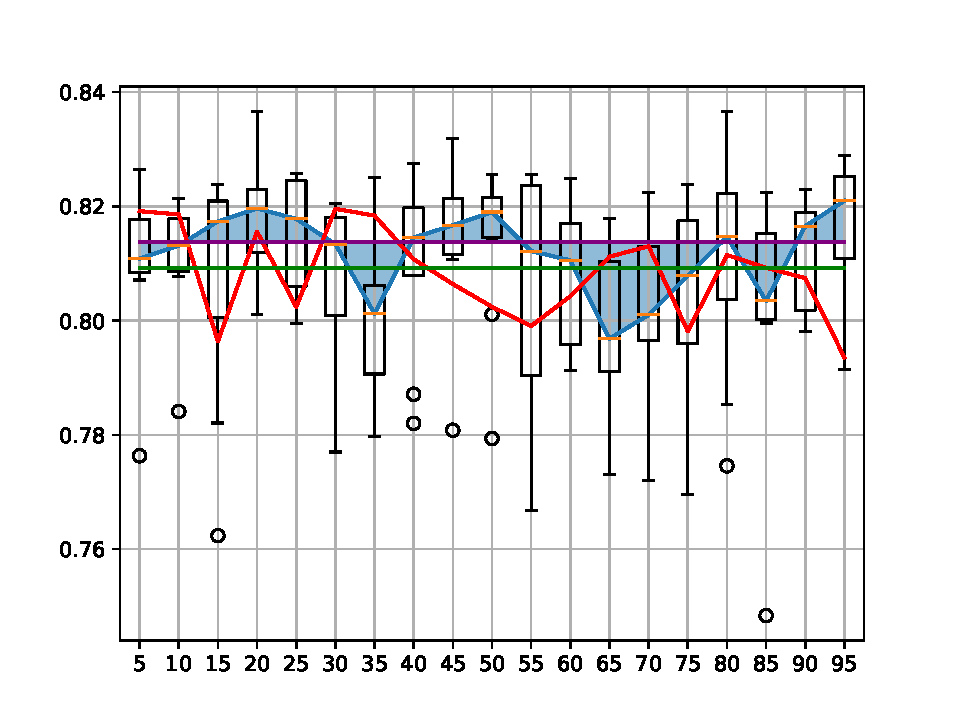
\includegraphics{cutoff-multi-1d-base-uni-100.pdf}
    % \includegraphics{cutoff-multi-1d-100-mean.pdf}
    \caption{Comparison between 1D KDEs (red) and multi-KDE (blue and boxplot) for different cutoffs. The $y$-axis shows the accuracy scores, and the purple line is the accuracy for the default configuration. The boxplot belongs to the multi-KDE model, and the lines show median score of 10 iterations (on each iteration 100 datasets were examined). The green line belongs to uniform sampling.}
    \label{fig:cutoff}
\end{figure}

\bibliographystyle{siam}
\bibliography{references.bib}

\end{document}
